\documentclass[a4paper, 11pt]{article}
\usepackage{comment} % enables the use of multi-line comments (\ifx \fi) 
\usepackage{lipsum} %This package just generates Lorem Ipsum filler text. 
\usepackage{fullpage} % changes the margin
\usepackage{tikz}
\usetikzlibrary{arrows,automata,positioning}
\usepackage[utf8]{inputenc}

\begin{document}
%Header-Make sure you update this information!!!!
\noindent
\large\textbf{Lenguajes Formales y Autómatas/Proyecto} \hfill \textbf{Integrantes del grupo:} \\
\normalsize INF - 154 \hfill Jhonatan Ismael Castro Rocabado\\
Profesora. Madelina Loza Soliz \hfill Fabiola Vanessa Aliaga Salvatierra\\
Periodo: Curso de Invierno 2016 \hfill Carlos Fernando Torrez Alanoca\\
\hfill Fecha: 24/7/2016 \\

\section*{Enunciado del Problema}
Realizar un autómata que acepte enunciados de operaciones algebraicas simples.

\section*{Autómata}

\subsection*{var++, var + var, var+=}

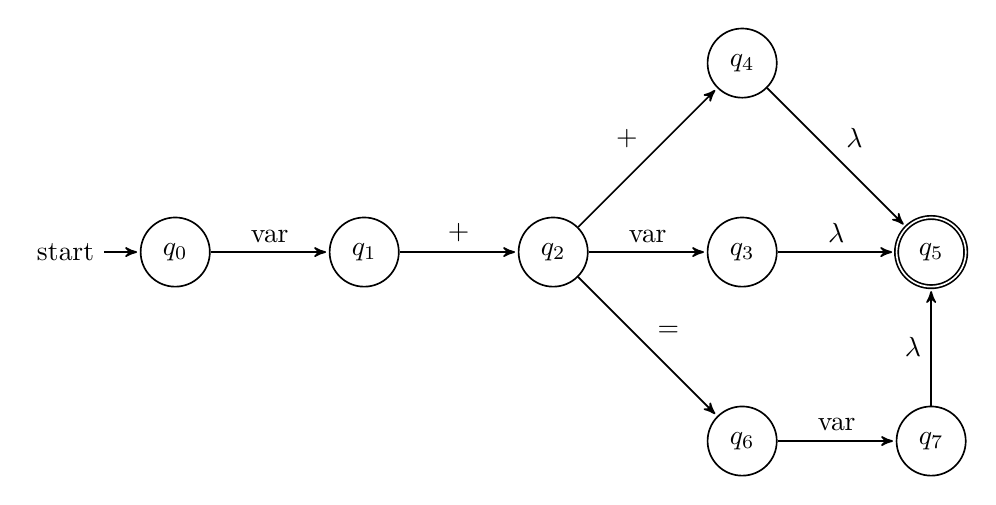
\begin{tikzpicture}[->,>=stealth',shorten >=1pt,auto,node distance=2.4cm,semithick]
  \tikzstyle{every state}=[fill=none,draw=black,text=black]

  \node[initial,state] (q0)                    {$q_0$};
  \node[state]         (q1) [right of=q0] {$q_1$};
  \node[state]         (q2) [right of=q1] {$q_2$};
  \node[state]         (q3) [right of=q2] {$q_3$};
  \node[state]         (q4) [above of=q3] {$q_4$};
  \node[state,accepting]         (q5) [right of=q3] {$q_5$};
  \node[state]         (q6) [below of=q3] {$q_6$};
  \node[state]         (q7) [below of=q5] {$q_7$};

  \path
  (q0) edge node {var} (q1)
  (q1) edge node {+} (q2)
  (q2) edge node {var} (q3)
  edge node {+} (q4)
  edge node {=} (q6)
  (q3) edge node {$\lambda$} (q5)
  (q4) edge node {$\lambda$} (q5)
  (q6) edge node {var} (q7)
  (q7) edge node {$\lambda$} (q5);
\end{tikzpicture}

\subsection*{var$--$, var $-$ var, var$-=$}

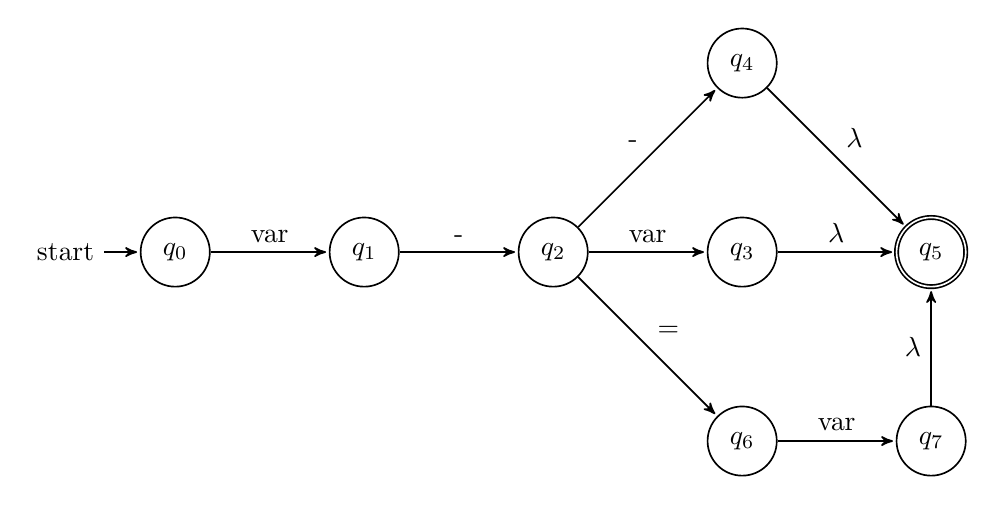
\begin{tikzpicture}[->,>=stealth',shorten >=1pt,auto,node distance=2.4cm,semithick]
  \tikzstyle{every state}=[fill=none,draw=black,text=black]

  \node[initial,state] (q0)                    {$q_0$};
  \node[state]         (q1) [right of=q0] {$q_1$};
  \node[state]         (q2) [right of=q1] {$q_2$};
  \node[state]         (q3) [right of=q2] {$q_3$};
  \node[state]         (q4) [above of=q3] {$q_4$};
  \node[state,accepting]         (q5) [right of=q3] {$q_5$};
  \node[state]         (q6) [below of=q3] {$q_6$};
  \node[state]         (q7) [below of=q5] {$q_7$};

  \path
  (q0) edge node {var} (q1)
  (q1) edge node {-} (q2)
  (q2) edge node {var} (q3)
  edge node {-} (q4)
  edge node {=} (q6)
  (q3) edge node {$\lambda$} (q5)
  (q4) edge node {$\lambda$} (q5)
  (q6) edge node {var} (q7)
  (q7) edge node {$\lambda$} (q5);
\end{tikzpicture}

\subsection*{var * var, var*=}

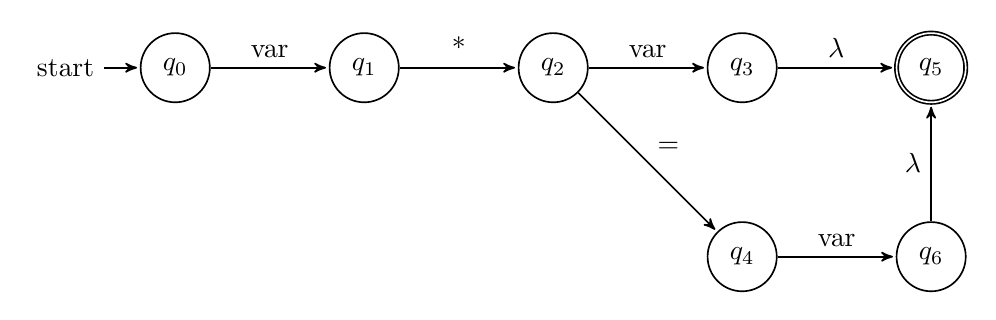
\begin{tikzpicture}[->,>=stealth',shorten >=1pt,auto,node distance=2.4cm,semithick]
  \tikzstyle{every state}=[fill=none,draw=black,text=black]

  \node[initial,state] (q0)                    {$q_0$};
  \node[state]         (q1) [right of=q0] {$q_1$};
  \node[state]         (q2) [right of=q1] {$q_2$};
  \node[state]         (q3) [right of=q2] {$q_3$};
  \node[state,accepting]         (q5) [right of=q3] {$q_5$};
  \node[state]         (q4) [below of=q3] {$q_4$};
  \node[state]         (q6) [below of=q5] {$q_6$};

  \path
  (q0) edge node {var} (q1)
  (q1) edge node {*} (q2)
  (q2) edge node {var} (q3)
  edge node {=} (q4)
  (q3) edge node {$\lambda$} (q5)
  (q4) edge node {var} (q6)
  (q6) edge node {$\lambda$} (q5);
\end{tikzpicture}

\subsection*{var / var, var/=}

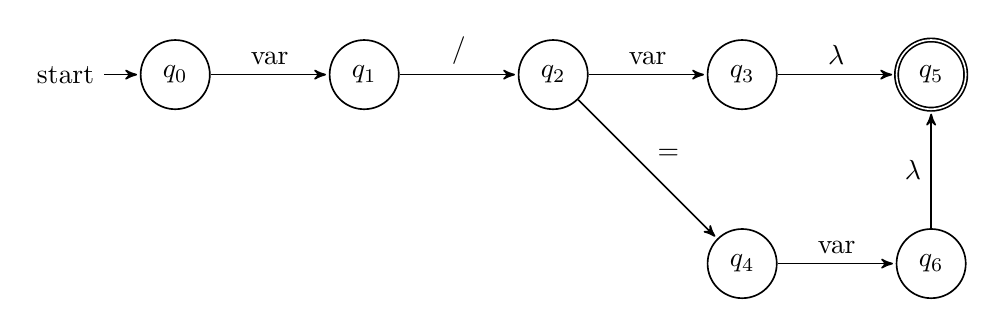
\begin{tikzpicture}[->,>=stealth',shorten >=1pt,auto,node distance=2.4cm,semithick]
  \tikzstyle{every state}=[fill=none,draw=black,text=black]

  \node[initial,state] (q0)                    {$q_0$};
  \node[state]         (q1) [right of=q0] {$q_1$};
  \node[state]         (q2) [right of=q1] {$q_2$};
  \node[state]         (q3) [right of=q2] {$q_3$};
  \node[state,accepting]         (q5) [right of=q3] {$q_5$};
  \node[state]         (q4) [below of=q3] {$q_4$};
  \node[state]         (q6) [below of=q5] {$q_6$};

  \path
  (q0) edge node {var} (q1)
  (q1) edge node {/} (q2)
  (q2) edge node {var} (q3)
  edge node {=} (q4)
  (q3) edge node {$\lambda$} (q5)
  (q4) edge node {var} (q6)
  (q6) edge node {$\lambda$} (q5);
\end{tikzpicture}

\subsection*{var \% var, var\%=}

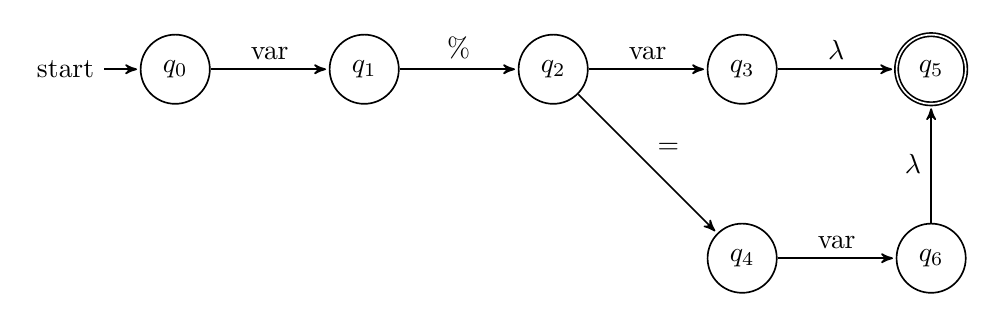
\begin{tikzpicture}[->,>=stealth',shorten >=1pt,auto,node distance=2.4cm,semithick]
  \tikzstyle{every state}=[fill=none,draw=black,text=black]

  \node[initial,state] (q0)                    {$q_0$};
  \node[state]         (q1) [right of=q0] {$q_1$};
  \node[state]         (q2) [right of=q1] {$q_2$};
  \node[state]         (q3) [right of=q2] {$q_3$};
  \node[state,accepting]         (q5) [right of=q3] {$q_5$};
  \node[state]         (q4) [below of=q3] {$q_4$};
  \node[state]         (q6) [below of=q5] {$q_6$};

  \path
  (q0) edge node {var} (q1)
  (q1) edge node {\%} (q2)
  (q2) edge node {var} (q3)
  edge node {=} (q4)
  (q3) edge node {$\lambda$} (q5)
  (q4) edge node {var} (q6)
  (q6) edge node {$\lambda$} (q5);
\end{tikzpicture}

\subsection*{var\&\&, var \& var, var\&=}

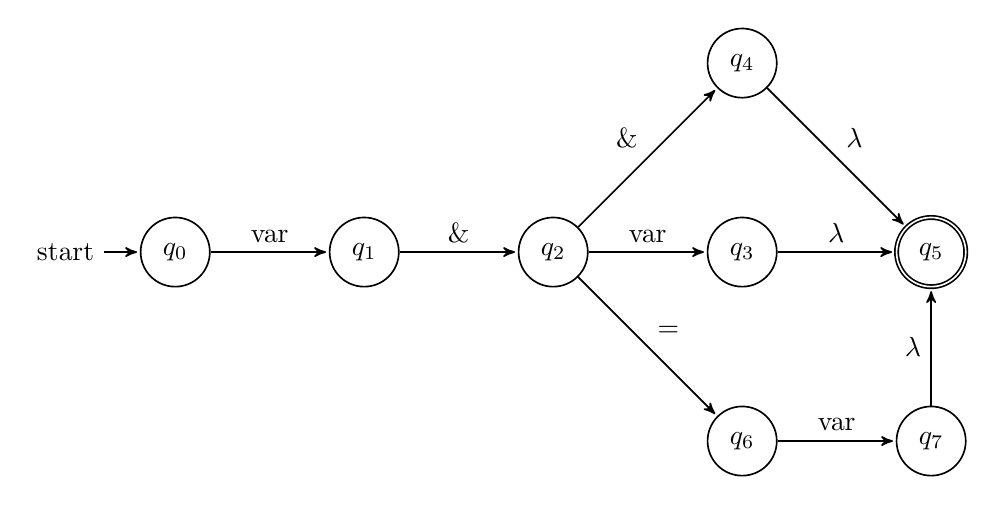
\begin{tikzpicture}[->,>=stealth',shorten >=1pt,auto,node distance=2.4cm,semithick]
  \tikzstyle{every state}=[fill=none,draw=black,text=black]

  \node[initial,state] (q0)                    {$q_0$};
  \node[state]         (q1) [right of=q0] {$q_1$};
  \node[state]         (q2) [right of=q1] {$q_2$};
  \node[state]         (q3) [right of=q2] {$q_3$};
  \node[state]         (q4) [above of=q3] {$q_4$};
  \node[state,accepting]         (q5) [right of=q3] {$q_5$};
  \node[state]         (q6) [below of=q3] {$q_6$};
  \node[state]         (q7) [below of=q5] {$q_7$};

  \path
  (q0) edge node {var} (q1)
  (q1) edge node {\&} (q2)
  (q2) edge node {var} (q3)
  edge node {\&} (q4)
  edge node {=} (q6)
  (q3) edge node {$\lambda$} (q5)
  (q4) edge node {$\lambda$} (q5)
  (q6) edge node {var} (q7)
  (q7) edge node {$\lambda$} (q5);
\end{tikzpicture}

\subsection*{var$||$, var $|$ var, var$|$=}

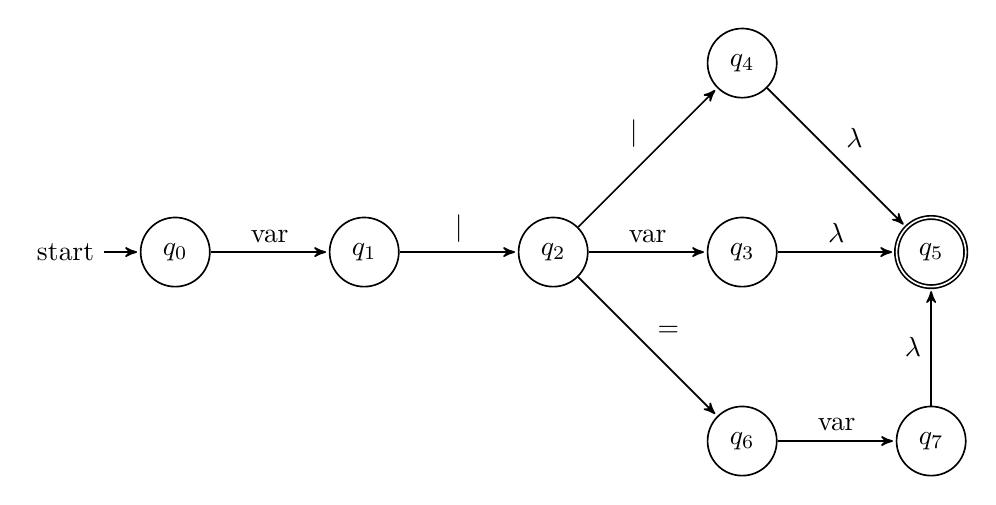
\begin{tikzpicture}[->,>=stealth',shorten >=1pt,auto,node distance=2.4cm,semithick]
  \tikzstyle{every state}=[fill=none,draw=black,text=black]

  \node[initial,state] (q0)                    {$q_0$};
  \node[state]         (q1) [right of=q0] {$q_1$};
  \node[state]         (q2) [right of=q1] {$q_2$};
  \node[state]         (q3) [right of=q2] {$q_3$};
  \node[state]         (q4) [above of=q3] {$q_4$};
  \node[state,accepting]         (q5) [right of=q3] {$q_5$};
  \node[state]         (q6) [below of=q3] {$q_6$};
  \node[state]         (q7) [below of=q5] {$q_7$};

  \path
  (q0) edge node {var} (q1)
  (q1) edge node {$|$} (q2)
  (q2) edge node {var} (q3)
  edge node {$|$} (q4)
  edge node {=} (q6)
  (q3) edge node {$\lambda$} (q5)
  (q4) edge node {$\lambda$} (q5)
  (q6) edge node {var} (q7)
  (q7) edge node {$\lambda$} (q5);
\end{tikzpicture}

\subsection*{var \^{} var, var\^{}=}

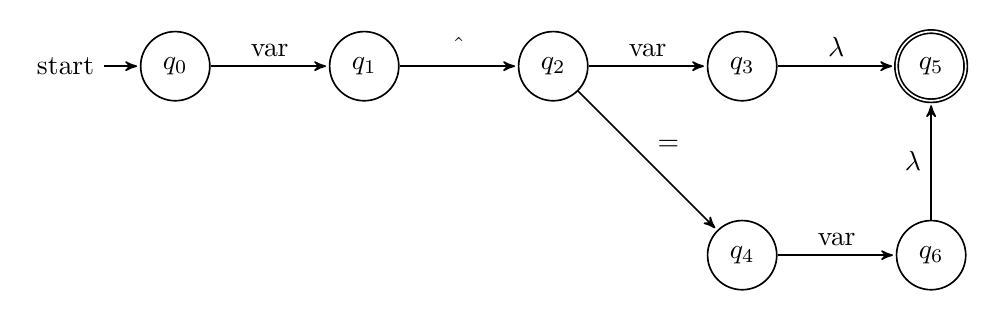
\begin{tikzpicture}[->,>=stealth',shorten >=1pt,auto,node distance=2.4cm,semithick]
  \tikzstyle{every state}=[fill=none,draw=black,text=black]

  \node[initial,state] (q0)                    {$q_0$};
  \node[state]         (q1) [right of=q0] {$q_1$};
  \node[state]         (q2) [right of=q1] {$q_2$};
  \node[state]         (q3) [right of=q2] {$q_3$};
  \node[state,accepting]         (q5) [right of=q3] {$q_5$};
  \node[state]         (q4) [below of=q3] {$q_4$};
  \node[state]         (q6) [below of=q5] {$q_6$};

  \path
  (q0) edge node {var} (q1)
  (q1) edge node {\^{}} (q2)
  (q2) edge node {var} (q3)
  edge node {=} (q4)
  (q3) edge node {$\lambda$} (q5)
  (q4) edge node {var} (q6)
  (q6) edge node {$\lambda$} (q5);
\end{tikzpicture}

\subsection*{var $<$ var, var $<=$ var, var $<<$ var, var $<<=$ var}

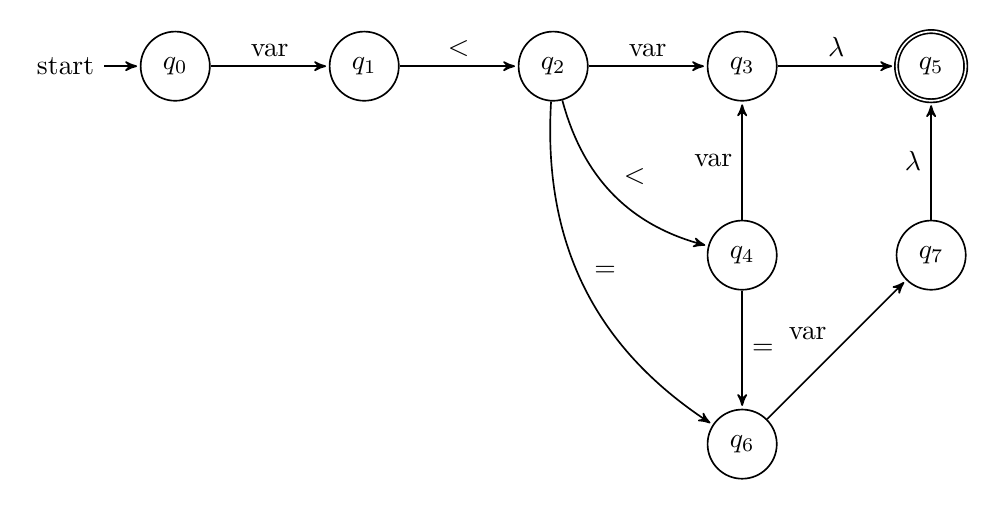
\begin{tikzpicture}[->,>=stealth',shorten >=1pt,auto,node distance=2.4cm,semithick]
  \tikzstyle{every state}=[fill=none,draw=black,text=black]

  \node[initial,state] (q0)                    {$q_0$};
  \node[state]         (q1) [right of=q0] {$q_1$};
  \node[state]         (q2) [right of=q1] {$q_2$};
  \node[state]         (q3) [right of=q2] {$q_3$};
  \node[state]         (q4) [below of=q3] {$q_4$};
  \node[state,accepting]         (q5) [right of=q3] {$q_5$};
  \node[state]         (q6) [below of=q4] {$q_6$};
  \node[state]         (q7) [below of=q5] {$q_7$};

  \path
  (q0) edge node {var} (q1)
  (q1) edge node {$<$} (q2)
  (q2) edge node {var} (q3)
  edge [bend right] node {$<$} (q4)
  edge [bend right] node {=} (q6)
  (q3) edge node {$\lambda$} (q5)
  (q4) edge node {var} (q3)
  edge node {$=$} (q6)
  (q6) edge node {var} (q7)
  (q7) edge node {$\lambda$} (q5);
\end{tikzpicture}

\subsection*{var $>$ var, var $>=$ var, var $>>$ var, var $>>=$ var, var $>>>=$ var}

\begin{tikzpicture}[->,>=stealth',shorten >=1pt,auto,node distance=3cm,semithick]
  \tikzstyle{every state}=[fill=none,draw=black,text=black]

  \node[initial,state] (q0)                    {$q_0$};
  \node[state]         (q1) [right of=q0] {$q_1$};
  \node[state]         (q2) [right of=q1] {$q_2$};
  \node[state]         (q3) [right of=q2] {$q_3$};
  \node[state]         (q4) [below of=q3] {$q_4$};
  \node[state,accepting]         (q5) [right of=q3] {$q_5$};
  \node[state]         (q6) [below of=q4] {$q_6$};
  \node[state]         (q7) [below of=q5] {$q_7$};
  \node[state]         (q8) [below of=q6] {$q_8$};
  

  \path
  (q0) edge node {var} (q1)
  (q1) edge node {$>$} (q2)
  (q2) edge node {var} (q3)
  edge [bend right] node {$>$} (q4)
  edge [bend right] node {=} (q8)
  (q3) edge node {$\lambda$} (q5)
  (q4) edge node {var} (q3)
  edge node {$>$} (q6)
  edge [bend right] node {$=$} (q8)
  (q6) edge node {=} (q8)
  (q8) edge node {var} (q7)
  (q7) edge node {$\lambda$} (q5);
\end{tikzpicture}

\subsection*{var $==$ var, var $!=$ var}

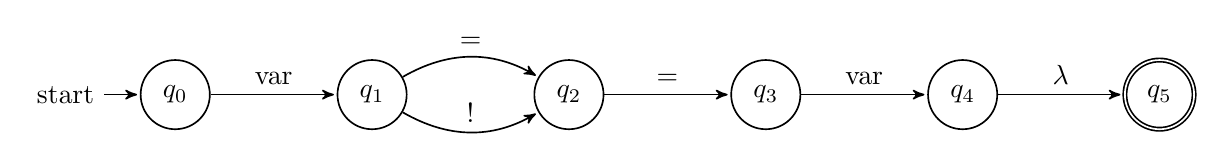
\begin{tikzpicture}[->,>=stealth',shorten >=1pt,auto,node distance=2.5cm,semithick]
  \tikzstyle{every state}=[fill=none,draw=black,text=black]

  \node[initial,state] (q0)                    {$q_0$};
  \node[state]         (q1) [right of=q0] {$q_1$};
  \node[state]         (q2) [right of=q1] {$q_2$};
  \node[state]         (q3) [right of=q2] {$q_3$};
  \node[state]         (q4) [right of=q3] {$q_4$};
  \node[state, accepting]         (q5) [right of=q4] {$q_5$};

  \path
  (q0) edge node {var} (q1)
  (q1) edge [bend left] node {=} (q2)
  edge [bend right] node {!} (q2)
  (q2) edge node {=} (q3)
  (q3) edge node {var} (q4)
  (q4) edge node {$\lambda$} (q5);
\end{tikzpicture}

\subsection*{$++$var, $+$var}

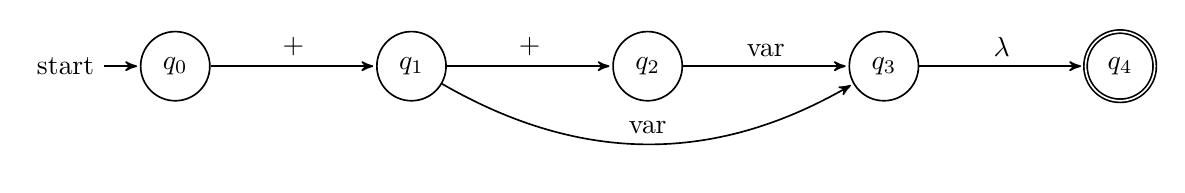
\begin{tikzpicture}[->,>=stealth',shorten >=1pt,auto,node distance=3cm,semithick]
  \tikzstyle{every state}=[fill=none,draw=black,text=black]

  \node[initial,state] (q0)                    {$q_0$};
  \node[state]         (q1) [right of=q0] {$q_1$};
  \node[state]         (q2) [right of=q1] {$q_2$};
  \node[state]         (q3) [right of=q2] {$q_3$};
  \node[state, accepting]         (q4) [right of=q3] {$q_4$};

  \path
  (q0) edge node {+} (q1)
  (q1) edge node {+} (q2)
  edge [bend right] node {var} (q3)
  (q2) edge node {var} (q3)
  (q3) edge node {$\lambda$} (q4);
\end{tikzpicture}

\subsection*{$--$var, $-$var}

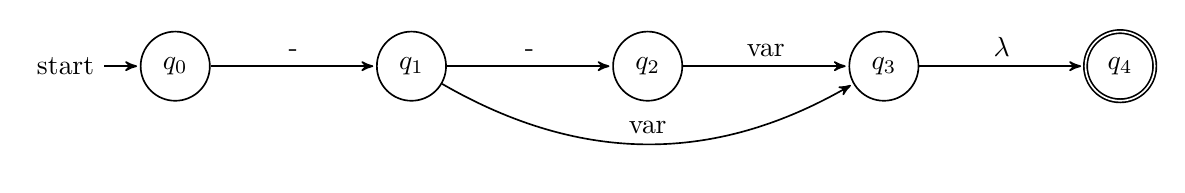
\begin{tikzpicture}[->,>=stealth',shorten >=1pt,auto,node distance=3cm,semithick]
  \tikzstyle{every state}=[fill=none,draw=black,text=black]

  \node[initial,state] (q0)                    {$q_0$};
  \node[state]         (q1) [right of=q0] {$q_1$};
  \node[state]         (q2) [right of=q1] {$q_2$};
  \node[state]         (q3) [right of=q2] {$q_3$};
  \node[state, accepting]         (q4) [right of=q3] {$q_4$};

  \path
  (q0) edge node {-} (q1)
  (q1) edge node {-} (q2)
  edge [bend right] node {var} (q3)
  (q2) edge node {var} (q3)
  (q3) edge node {$\lambda$} (q4);
\end{tikzpicture}

\subsection*{$!$ var}

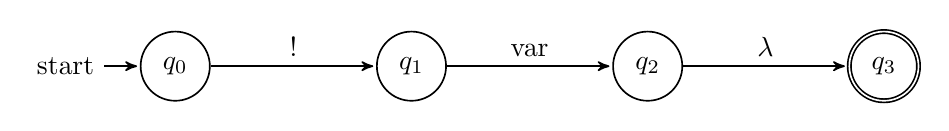
\begin{tikzpicture}[->,>=stealth',shorten >=1pt,auto,node distance=3cm,semithick]
  \tikzstyle{every state}=[fill=none,draw=black,text=black]

  \node[initial,state] (q0)                    {$q_0$};
  \node[state]         (q1) [right of=q0] {$q_1$};
  \node[state]         (q2) [right of=q1] {$q_2$};
  \node[state, accepting]         (q3) [right of=q2] {$q_3$};

  \path
  (q0) edge node {$!$} (q1)
  (q1) edge node {var} (q2)
  (q2) edge node {$\lambda$} (q3);
\end{tikzpicture}

\subsection*{$\sim$ var}

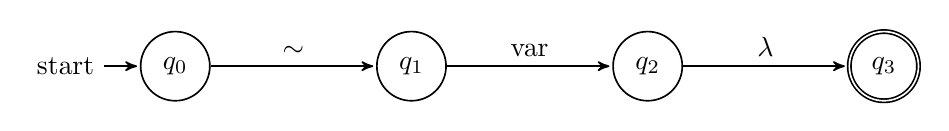
\begin{tikzpicture}[->,>=stealth',shorten >=1pt,auto,node distance=3cm,semithick]
  \tikzstyle{every state}=[fill=none,draw=black,text=black]

  \node[initial,state] (q0)                    {$q_0$};
  \node[state]         (q1) [right of=q0] {$q_1$};
  \node[state]         (q2) [right of=q1] {$q_2$};
  \node[state, accepting]         (q3) [right of=q2] {$q_3$};

  \path
  (q0) edge node {$\sim$} (q1)
  (q1) edge node {var} (q2)
  (q2) edge node {$\lambda$} (q3);
\end{tikzpicture}

\subsection*{condition ? statement : statement}

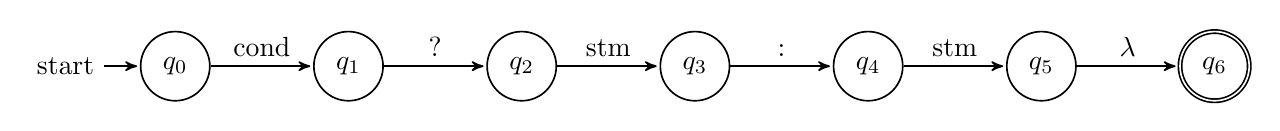
\begin{tikzpicture}[->,>=stealth',shorten >=1pt,auto,node distance=2.2cm,semithick]
  \tikzstyle{every state}=[fill=none,draw=black,text=black]

  \node[initial,state] (q0)                    {$q_0$};
  \node[state]         (q1) [right of=q0] {$q_1$};
  \node[state]         (q2) [right of=q1] {$q_2$};
  \node[state]         (q3) [right of=q2] {$q_3$};
  \node[state]         (q4) [right of=q3] {$q_4$};
  \node[state]         (q5) [right of=q4] {$q_5$};
  \node[state, accepting]         (q6) [right of=q5] {$q_6$};

  \path
  (q0) edge node {cond} (q1)
  (q1) edge node {?} (q2)
  (q2) edge node {stm} (q3)
  (q3) edge node {:} (q4)
  (q4) edge node {stm} (q5)
  (q5) edge node {$\lambda$} (q6);
\end{tikzpicture}

\section*{Operadores de Java}

\begin{center}
  \includegraphics[scale=0.5]{java_operators}
\end{center}

Esta información fue obtenida de la documentación ofical de Java. \cite{java}

\begin{thebibliography}{9}
\bibitem{java} https://docs.oracle.com/javase/tutorial/java/nutsandbolts/operators.html
\end{thebibliography}

\end{document}
